\section{Power spectrum metric}

The second task of the project was to implement the power-spectrum correlation (PSC). This features two hyperparameters: Namely
\begin{itemize}
	\item the smoothing factor $\sigma$, which is the width of the Gaussian kernel smoothing the spectrum
	\item and the cutoff, which excludes all frequencies above the given frequency threshold from the calculation of the power spectrum correlation.
\end{itemize}
The code snippets of \textit{psc.py} was added in \textit{global\_utils.py} and executed in \textit{rnn\_statefull.py}. Furthermore the plotting functions are added in the \textit{plotting\_utils.py} file.
In order to ensure that the model draws a random initial condition and then generates a time series of length T. We sampled random indices in the data generation and for each prediction the model takes one of these random integers during testing. And starts to predict the time series starting at the chosen starting point of the whole test series.

To illustrate the LSTM model and also to make sure whether the LSTM model is working, we first apply the model on a very simple sinosoidal dataset before applying it on the Lorenz datasets (see \cref{sec3}). For this we generate a time series consisting of 100000 points with time step size $\Delta t=0.5$ by computing:
\begin{align}
	z_t = A\cdot\sin(2\pi ft+\phi_0)+c
\end{align}
The chosen parameters are:
\begin{itemize}
	\setlength\itemsep{0.1em}
	\item amplitude $A = 2$
	\item frequency $f = 0.1$
	\item phase $\phi_0^{\text{train}}=0$, $\phi_0^{\text{test}}=0.5$
	\item offset $c=0.5$
\end{itemize}

Using the implemented LSTM Model of Vlachas et alium \cite{Vlachas}\footnote{\url{https://github.com/pvlachas/RNN-RC-Chaos}} one can train the LSTM model and test the LSTM model via the command line. The root mean squared error is chosen to be the loss, which is optimized during training. The loss decreases with increasing epochs for the training data and the validation data as well. This can be seen in \cref{2:loss}. Since validation loss is not increasing one can exclude the existence of overfitting.
\begin{figure}[h]
	\centering
	\begin{subfigure}[b]{0.45\textwidth}
		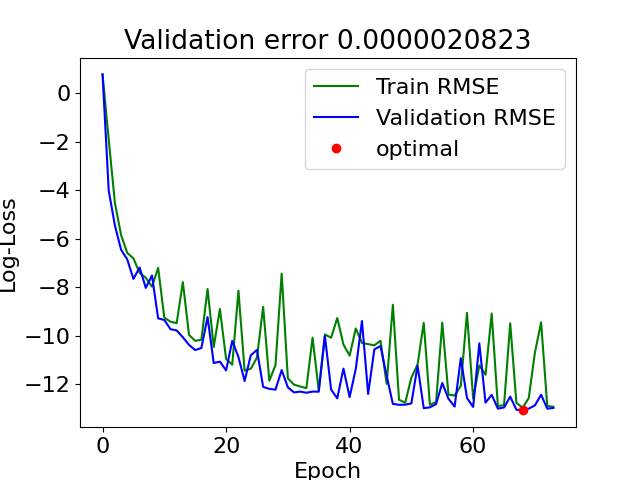
\includegraphics[width=\textwidth]{../Results/Test-Task02/Figures/RNN-lstm-RDIM_1-N_used_50000-NUM-LAY_1-SIZE-LAY_100-ACT_tanh-ISH_statefull-SL_8-PL_4-LR_0.001-DKP_1.0-ZKP_1.0-HSPL_300-IPL_200-NL_1-WID_0/Loss_total_log.png}
		\caption{Training and validation loss}
		\label{2:loss}
	\end{subfigure}
	\begin{subfigure}[b]{0.45\textwidth}
		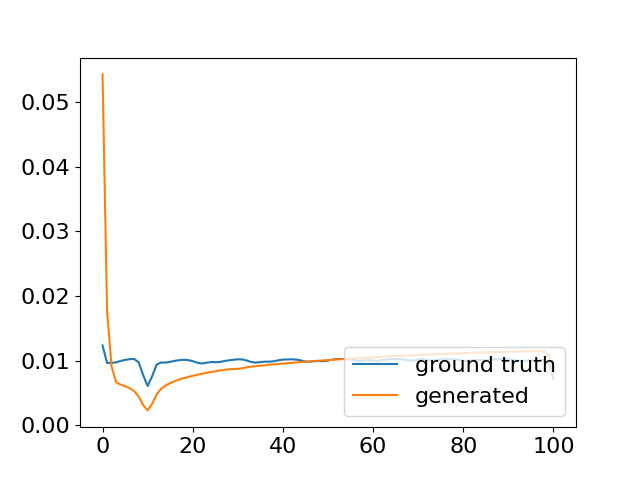
\includegraphics[width=\textwidth]{../Results/Test-Task02/Figures/RNN-lstm-RDIM_1-N_used_50000-NUM-LAY_1-SIZE-LAY_100-ACT_tanh-ISH_statefull-SL_8-PL_4-LR_0.001-DKP_1.0-ZKP_1.0-HSPL_300-IPL_200-NL_1-WID_0/spectrum_comparison_TEST.png}
		\caption{Power spectrum for test predictions}
		\label{2:spectrum}
	\end{subfigure}
\end{figure}

The plotted power spectrum shows a clear negative peak at 10, which corresponds to the chosen frequency of 0.1. %\textcolor{red}{\textbf{at ziqiu: do you know what the unit of the x-axis is?}}.
The power spectrum of the generated predictions show the same course of the curve as the ground truth, but appearently is shifted a bit. For the power spectrum plot we used a smoothing factor $\sigma=1$ and a frequency cutoff at 5000.

\FloatBarrier
Furthermore in \cref{2:predictions1} and \cref{2:predictions2} one can see the predictions of the LSTM of two test series with random chosen initial conditions and the corresponding errors. One can see that the LSTM can easily extract the sinosoidal behavior of the system and is able to fit to the data very well. However, one can see that the curves are a little bit off. Probably because the regressed frequency is not optimally. This explains why the error is increasing and accumulating the more the model predicts in the future.
\begin{figure}[h]
	\centering
	\begin{subfigure}[b]{0.45\textwidth}
		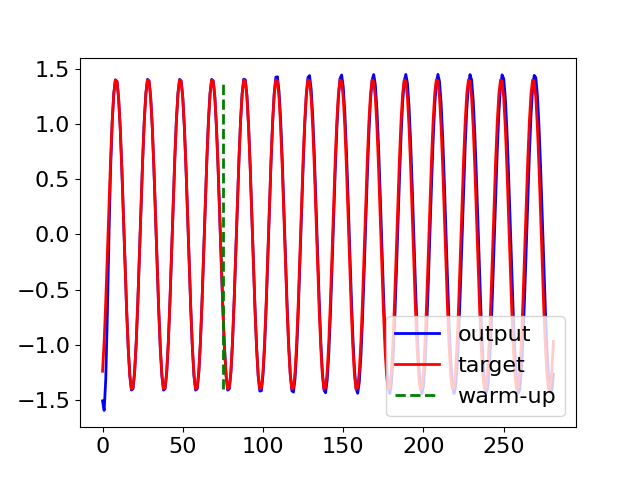
\includegraphics[width=\textwidth]{../Results/Test-Task02/Figures/RNN-lstm-RDIM_1-N_used_50000-NUM-LAY_1-SIZE-LAY_100-ACT_tanh-ISH_statefull-SL_8-PL_4-LR_0.001-DKP_1.0-ZKP_1.0-HSPL_300-IPL_200-NL_1-WID_0/prediction_augmend_TEST_70417.png}
		\caption{Prediction}
	\end{subfigure}
	\begin{subfigure}[b]{0.45\textwidth}
		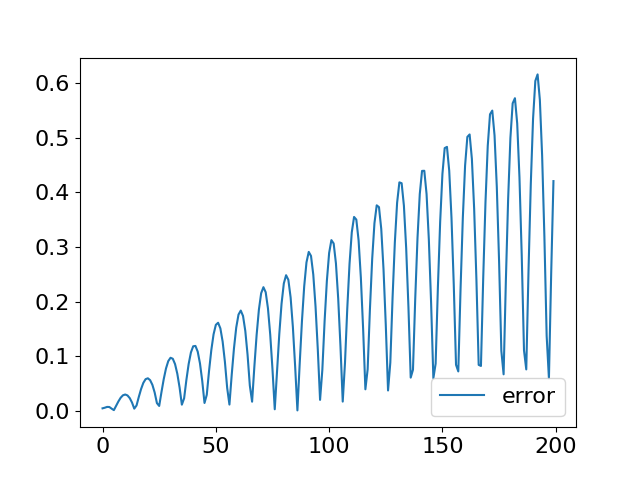
\includegraphics[width=\textwidth]{../Results/Test-Task02/Figures/RNN-lstm-RDIM_1-N_used_50000-NUM-LAY_1-SIZE-LAY_100-ACT_tanh-ISH_statefull-SL_8-PL_4-LR_0.001-DKP_1.0-ZKP_1.0-HSPL_300-IPL_200-NL_1-WID_0/prediction_TEST_70417_error.png}
		\caption{Error}
	\end{subfigure}
	\caption{Test results for random initial condition 70417}
	\label{2:predictions1}
\end{figure}
\begin{figure}[h]
	\centering
	\begin{subfigure}[b]{0.45\textwidth}
		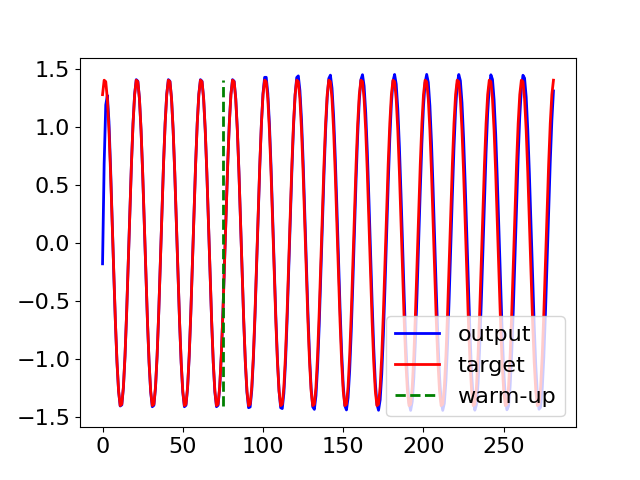
\includegraphics[width=\textwidth]{../Results/Test-Task02/Figures/RNN-lstm-RDIM_1-N_used_50000-NUM-LAY_1-SIZE-LAY_100-ACT_tanh-ISH_statefull-SL_8-PL_4-LR_0.001-DKP_1.0-ZKP_1.0-HSPL_300-IPL_200-NL_1-WID_0/prediction_augmend_TEST_98804.png}
		\caption{Prediction}
	\end{subfigure}
	\begin{subfigure}[b]{0.45\textwidth}
		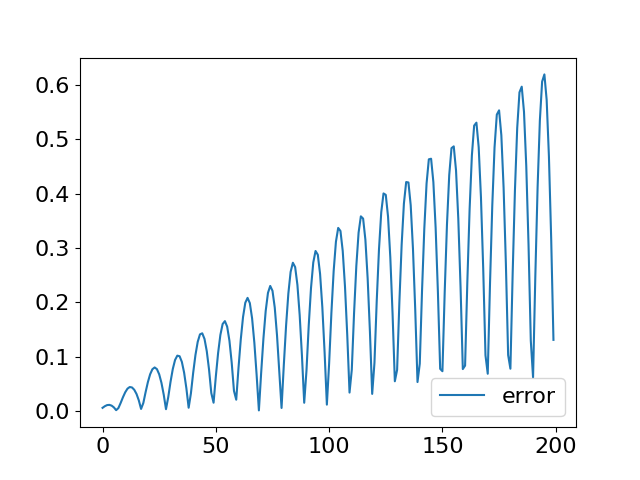
\includegraphics[width=\textwidth]{../Results/Test-Task02/Figures/RNN-lstm-RDIM_1-N_used_50000-NUM-LAY_1-SIZE-LAY_100-ACT_tanh-ISH_statefull-SL_8-PL_4-LR_0.001-DKP_1.0-ZKP_1.0-HSPL_300-IPL_200-NL_1-WID_0/prediction_TEST_98804_error.png}
		\caption{Error}
	\end{subfigure}
	\caption{Test results for random initial condition 98804}
	\label{2:predictions2}
\end{figure}

\newpage